\documentclass[12pt]{article}%
\usepackage{amsfonts}
\usepackage{fancyhdr}
\usepackage{xcolor}
\usepackage[a4paper, top=2.5cm, bottom=2.5cm, left=2.2cm, right=2.2cm]%
{geometry}
\usepackage{amsmath}
\usepackage{changepage}
\usepackage{amssymb}
\usepackage{graphicx}
\usepackage{inconsolata}
\usepackage{hyperref}
\hypersetup{
    colorlinks=true,
    linkcolor=blue,
    filecolor=magenta,      
    urlcolor=blue,
}
\usepackage{listings}
\setcounter{MaxMatrixCols}{30}
\newtheorem{theorem}{Theorem}
\newtheorem{acknowledgement}[theorem]{Acknowledgement}
\newtheorem{algorithm}[theorem]{Algorithm}
\newtheorem{axiom}{Axiom}
\newtheorem{case}[theorem]{Case}
\newtheorem{claim}[theorem]{Claim}
\newtheorem{conclusion}[theorem]{Conclusion}
\newtheorem{condition}[theorem]{Condition}
\newtheorem{conjecture}[theorem]{Conjecture}
\newtheorem{corollary}[theorem]{Corollary}
\newtheorem{criterion}[theorem]{Criterion}
\newtheorem{definition}[theorem]{Definition}
\newtheorem{example}[theorem]{Example}
\newtheorem{exercise}[theorem]{Exercise}
\usepackage{hyperref}

\usepackage{minted}
\newtheorem{lemma}[theorem]{Lemma}
\newtheorem{notation}[theorem]{Notation}
\newtheorem{problem}[theorem]{Problem}
\newtheorem{proposition}[theorem]{Proposition}
\newtheorem{remark}[theorem]{Remark}
\newtheorem{solution}[theorem]{Solution}
\newtheorem{summary}[theorem]{Summary}
\newenvironment{proof}[1][Proof]{\textbf{#1.} }{\ \rule{0.5em}{0.5em}}

\newcommand{\Q}{\mathbb{Q}}
\newcommand{\R}{\mathbb{R}}
\newcommand{\C}{\mathbb{C}}
\newcommand{\Z}{\mathbb{Z}}

\begin{document}

\title{Homework Assignment 3}
\author{CSE 151A: Introduction to Machine Learning}
\date{}
\maketitle

%%%% Deadline
\noindent \textbf {Due: May 10th, 2022, 9:30am (Pacific Time)} \\


%%%% Instructions.
\noindent \textbf {Instructions:} Please answer the questions below, attach your code in the document, and insert figures to create \textbf{a single PDF file}.\\

\noindent Grade: \underline{\hspace{.8cm}} out of 100 points 


\section{(20 points) SVM and kernel}
\begin{enumerate}
    \item (Linearly separability)(5 points) In lecture, we mentioned \textbf{Hard SVM} only works for \textbf{linearly separable} data points. Now you are given dataset $S=\left\{\left(\mathbf{x}_{i}, y_{i}\right), i=1, . ., N\right\}$ where each data point $(\mathbf{x}, y)$ contains a feature vector $\mathbf{x} \in \mathbb{R}^{2}$ and a label $y \in\{+,-\}$. Is the dataset linearly separable? If yes, please specify a decision boundary that linearly separates the data points with positive label from the data points with negative label.
    \begin{itemize}
        \item Case 1:\\
        \begin{table}[h]
            \centering
            \begin{tabular}{|c|c|}
                \hline label $(\mathrm{y})$ & features $(\mathbf{x})$ \\
                \hline Positive $(+)$ & $(0,0)$ \\
                \hline Negative $(-)$ & $(1,0),(0,1),(-1,0),(0,-1)$ \\
                \hline
            \end{tabular}
        \end{table}
        \\
        \\
        \\
        \item Case 2:\\
        \begin{table}[h]
            \centering
            \begin{tabular}{|c|c|}
                \hline label $(\mathrm{y})$ & features $(\mathbf{x})$ \\
                \hline Positive $(+)$ & $(0,1),(1,0)$ \\
                \hline Negative $(-)$ & $(-1,0),(0,-1)$ \\
                \hline
            \end{tabular}
        \end{table}
    \end{itemize}
    \newpage
    \item (Feature map and kernel)(10 points) Sometimes, data points that are not linearly separable in one feature space might be linearly separable in another. Therefore, we need a \textbf{transformation function (feature map)} $\phi$, that maps features from one space to another space. Suppose for feature vector $\mathbf{x}=\left(x_{1}, x_{2}\right) \in \mathbb{R}^{2}$ we define \textbf{feature map} $\phi: \mathbb{R}^{2} \rightarrow \mathbb{R}^{3}$ as: $\phi(\mathbf{x})=\left(x_{1}^{2}, x_{2}^{2}, \sqrt{2} x_{1} x_{2}\right)$. Given the \textbf{feature map} $\phi$, the corresponding \textbf{kernel} is defined as: $k(\mathbf{x}, \mathbf{z})=\phi(\mathbf{x}) \cdot \phi(\mathbf{z})$, where $\mathbf{x}, \mathbf{z} \in \mathbb{R}^{2}$. Prove that $k(\mathbf{x}, \mathbf{z})=(\mathbf{x} \cdot \mathbf{z})^{2}$ is the \textbf{kernel} for $\phi .$ In other words, prove that $\phi(\mathbf{x}) \cdot \phi(\mathbf{z})=(\mathbf{x} \cdot \mathbf{z})^{2}$.
    
    \textbf{Hint:} for vectors $\mathbf{x}, \mathbf{y} \in \mathbb{R}^{n}, \mathbf{x} \cdot \mathbf{y}=x_{1} y_{1}+x_{2} y_{2}+\ldots+x_{n} y_{n}$.
    \\
    \\
    \\
    \\
    \\
    \\
    \\
    \\
    \\
    \\
    \\
    \\

    \item (5 points) Recall Case 1 in part 1. Apply $\phi$ defined in part 2 to the 5 data points in Case 1 and compute the new features in $\mathbb{R}^{3}$. Are they now linearly separable in $\mathbb{R}^{3}$ ? (Optional: specify a valid decision boundary in $\mathbb{R}^{3}$ if linearly separable)
    
    \newpage

\end{enumerate}



\section{(10 points) K-means}

Suppose you are given 4 data points: $\mathbf{x}_{1}, \mathbf{x}_{2}, \mathbf{x}_{3}, \mathbf{x}_{4} \in \mathbb{R}^{2}$, where $\mathbf{x}_{1}=(1,0), \mathbf{x}_{2}=(1,1)$, $\mathbf{x}_{1}=(-1,0), \mathbf{x}_{1}=(-1,-1)$. Assume we know these points can be put into 2 clusters $(k$ $=2)$. Suppose we start with \textbf{centroids} $\mathbf{c}_{1}=(2,0), \mathbf{c}_{2}=(0,-1)$. Calculate where the new centroids would be after 1 iteration of \textbf{K-means}. Do the new centroids locations make sense?

\newpage


\section{(10 points) Gaussian Mixture Models}

Suppose we have a set of probabilistic clusters, $\mathbf{C}=\left(C_{1}, C_{2}\right) . C_{1}$ has probability density function $f_{1}=\mathcal{N}(0,1)$, that is, a Gaussian distribution with mean 0 and variance 1 , and $C_{2}$ has probability density function $f_{2}=\mathcal{N}(1,1)$. The weights of these clusters are given as: $\mathbb{P}\left(C_{1}\right)=\mathbb{P}\left(C_{2}\right)=0.5$. Given the following data points in $1 \mathrm{D}$, calculate the probability $\mathbb{P}(x \mid \mathbf{C})$ that a data point $x$ is generated by this set of clusters $\mathbf{C}$, for the following 2 data points: $(1) x=0.7,(2) x=1.5$.

Hint: The probability density function of $\mathcal{N}(\mu, \sigma)$ is: $f(x)=\frac{1}{\sigma \sqrt{2 \pi}} \exp \frac{-(x-\mu)^{2}}{2 \sigma^{2}}$

\newpage

\section{(10 points) Principle Component Analysis (PCA)}

You are now given some data points in 2D, with 2 kinds of labels (``+" and ``o").

\begin{figure}[h]
    \centering
    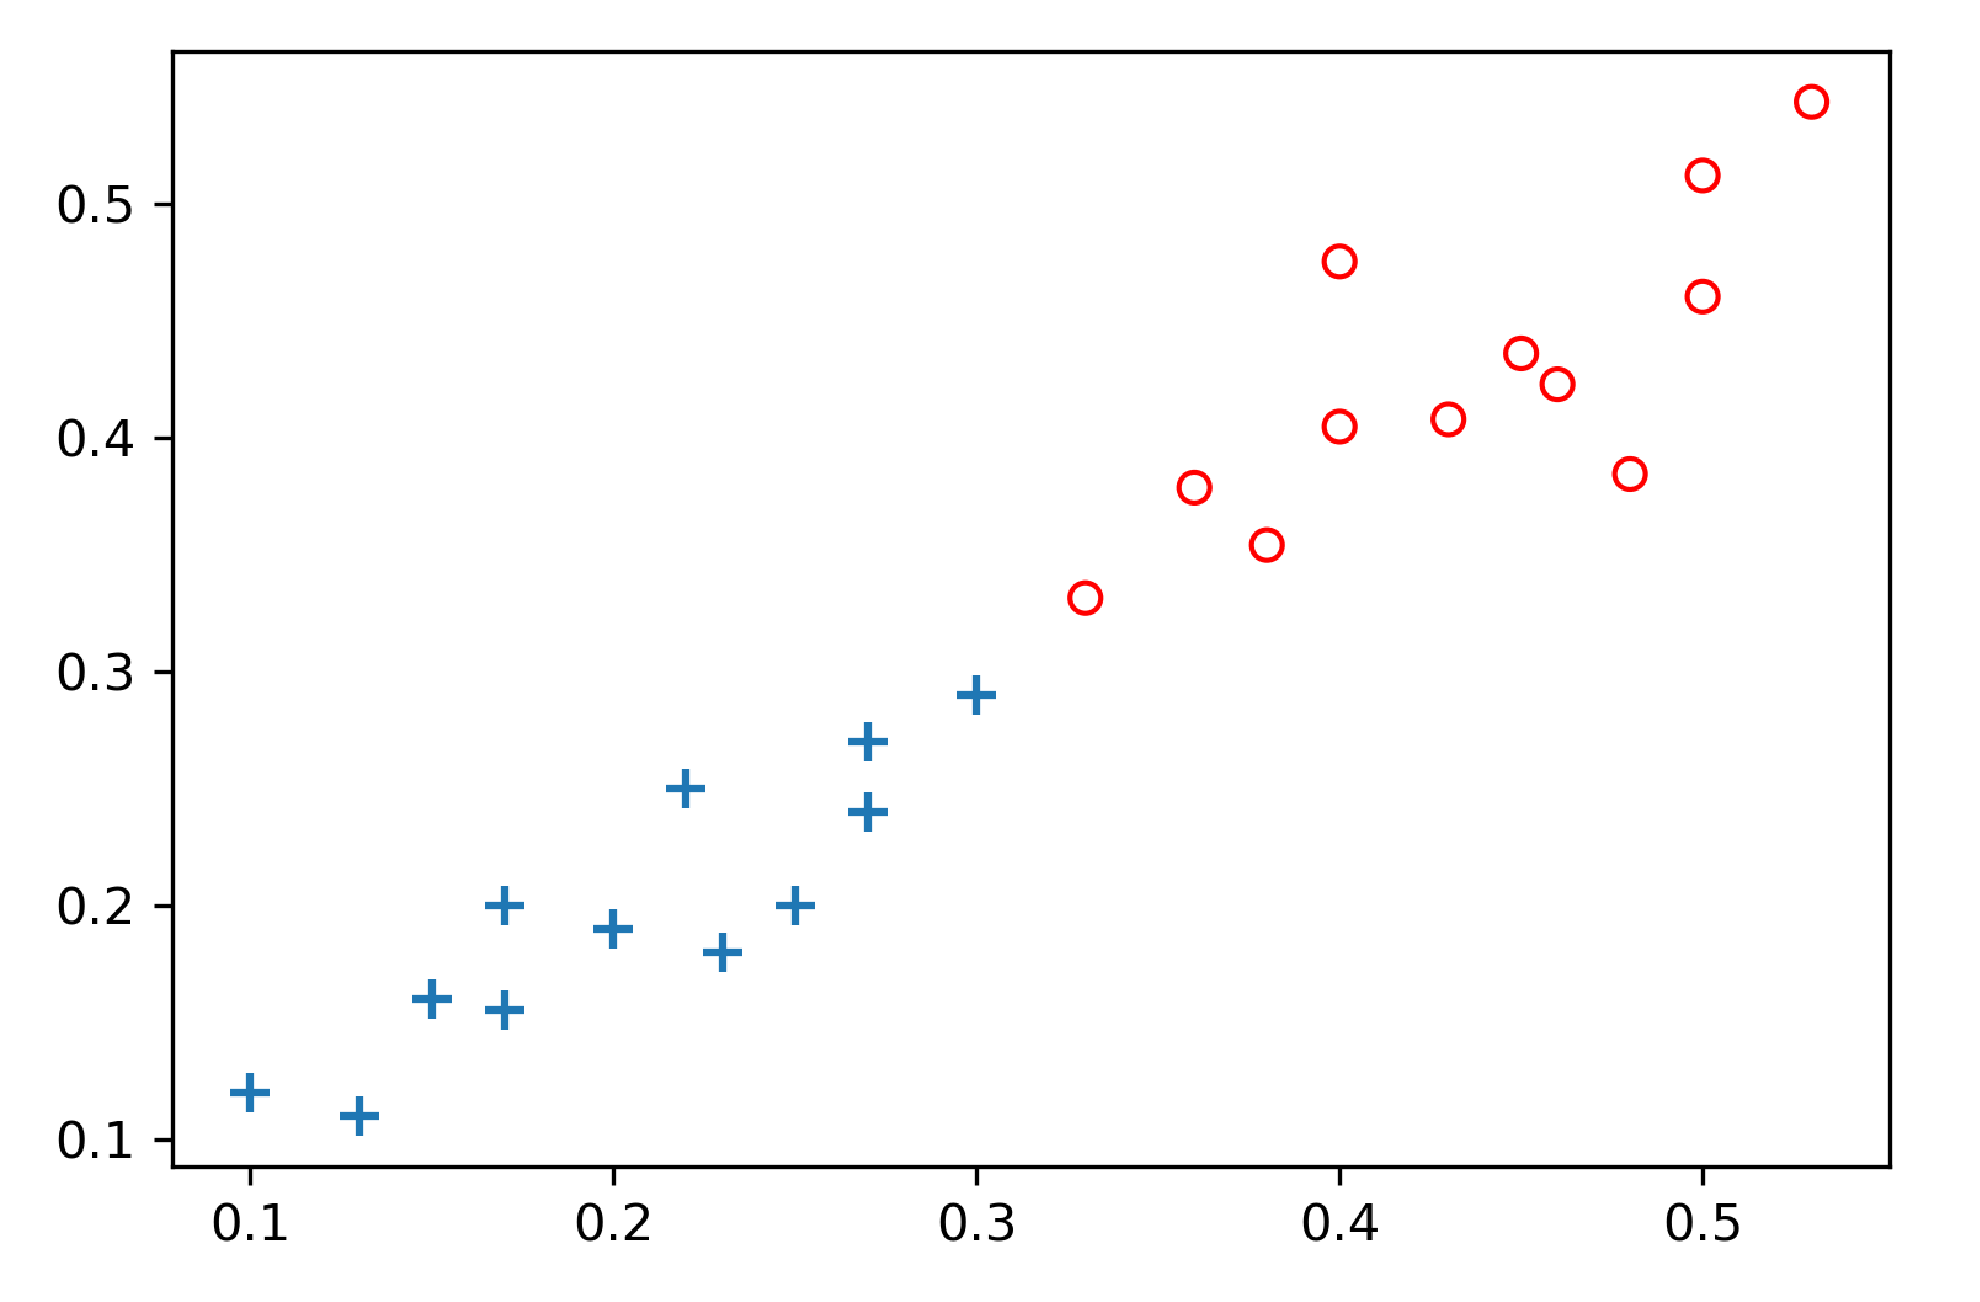
\includegraphics[width=0.6\linewidth]{fig.png}
\end{figure}

(1) (5 points) On the scatter plot, roughly draw the direction for the $1^{\text {st }}$ and $2^{\text {nd }}$ principle axes for this dataset.

(2) (5 points) Which principle axis would you choose to project onto, if we want to project the $2 \mathrm{D}$ features onto $1 \mathrm{D}$, and still want good separation between the 2 labels?

\newpage

\section{(50 points) Implementing the K-means algorithm}

Now, you will implement a K-Means model from scratch. We have provided a skeleton code file (i.e. KMeans.py) for you to implement the algorithm as well as a notebook file (i.e. KMeans.ipynb) for you to conduct experiments and answer relevant questions. Libraries such as numpy and pandas may be used for auxiliary tasks (such as matrix multiplication, matrix inversion, and so on), but not for the algorithms. That is, you can use numpy to implement your model, but cannot directly call libraries such as scikit-learn to get a K-Means model for your skeleton code. We will grade this question based on the three following criteria:

\begin{enumerate}
    \item Your implementation in code. Please do not change the structure of our skeleton code.
    \item Your model’s performance (we check if your model behaves correctly based on the results from multiple experiments in the notebook file).
    \item Your written answers for questions in the notebook file.
\end{enumerate}


\end{document}